\chapter{Biểu diễn màu, hadron và sự giam hãm}

\paragraph{Một đoạn dừng ngắn mở đầu.}
Trước khi quay lại lý thuyết nhóm, xin cho phép một lời quảng cáo trơ trẽn. \emph{The
Black Hole War} kể câu chuyện về cuộc tranh luận kéo dài với Stephen Hawking về việc liệu hố đen có phá hủy thông tin lượng tử hay không. Nó cũng ghi lại phần nào sự tàn nhẫn rất riêng của các nhà vật lý lý thuyết: không chỉ con mèo của Schrodinger, mà cả những con cá của Susskind và chuyến đi xui xẻo của chúng xuống bồn cầu. Xong nghĩa vụ đó, ta quay lại với Alice và Bob. Alice vẫn đang khổ sở, vì Bob vẫn bắt cô ấy học lý thuyết nhóm.

\lectureoverview{Một đối xứng trở thành vật lý thông qua tác dụng của nó lên các trạng thái. Ta bắt đầu với các phép quay để giới thiệu các biểu diễn và các toán tử sinh, rồi lặp lại cấu trúc đó cho màu \(SU(3)\). Các biểu diễn màu kết hợp thành các hadron, và động lực học của chúng giải thích vì sao không bao giờ quan sát thấy màu cô lập.}

\section{Nhóm và các đối tượng mà nó tác dụng lên}

Trong mọi thảo luận về đối xứng đều có hai ý niệm. Thứ nhất là một nhóm trừu tượng: một tập hợp các phép toán với luật nhân, phần tử đơn vị và các phần tử nghịch đảo. Thứ hai là các đối tượng mà những phép toán ấy tác dụng lên. Có thể phân biệt hai ý niệm này, nhưng trong vật lý thì không thể tách chúng rời nhau. Một đối xứng có ý nghĩa vì nó biến đổi các trạng thái vật lý, các trường, các tọa độ hoặc các đại lượng quan sát được.

\begin{classroomqa}
\audiencequestion{Một nhóm vừa được mô tả như một bảng nhân trừu tượng, vừa như các ma trận tác dụng lên các đối tượng vật lý. Hai phần đó có thể tách rời nhau không?
\lecturetimestamp{00:01:58}}
\lecturerresponse{Đó là hai mức mô tả khác nhau, nhưng chúng liên hệ hoàn toàn với nhau. Một phép quay tồn tại như một phép toán trừu tượng trước khi ta chỉ rõ nó quay cái gì. Khi đó vật lý hỏi chính phép toán ấy tác dụng thế nào lên các trạng thái và các đại lượng thích hợp với một hệ cụ thể. Các ma trận cung cấp tác dụng cụ thể đó đồng thời vẫn bảo toàn luật nhân trừu tượng.}
\end{classroomqa}

Các phép quay trong không gian cho ví dụ sáng sủa nhất. Trong cơ học cổ điển, cùng một phép quay có thể tác dụng lên tọa độ của hạt, lên phương của một nam châm, hoặc lên bất kỳ vectơ nào khác. Trong cơ học lượng tử, các trạng thái sống trong một không gian vectơ tuyến tính, nên một phép quay được biểu diễn bởi một toán tử tuyến tính trên không gian đó. Nếu \(g\) ký hiệu một phần tử nhóm trừu tượng và \(D(g)\) là đại diện ma trận của nó, thì tính nhất quán có nghĩa là
\begin{equation}
D(g_1g_2)=D(g_1)D(g_2),
\qquad
D(e)=\boldsymbol 1.
\end{equation}
Các ma trận không nhất thiết phải trông giống các phép toán trừu tượng, nhưng phép nhân của chúng phải tái tạo phép nhân của nhóm.
\editorialnote{Phương trình đồng cấu này viết tường minh sự tương ứng giữa phép nhân nhóm và phép nhân ma trận đã được mô tả bằng lời trong nguồn.}

Kích thước của ma trận được quyết định bởi không gian trạng thái, chứ không chỉ bởi riêng nhóm trừu tượng. Nếu ta chỉ giữ lại spin của một electron, có hai khả năng trực giao, spin lên và spin xuống, và một trạng thái là một vectơ cột hai thành phần. Vì thế các phép quay tác dụng thông qua các ma trận \(2\times2\). Đối với hai đối tượng spin một phần hai, có bốn trạng thái cơ sở,
\begin{equation}
\ket{\uparrow\uparrow},\qquad
\ket{\uparrow\downarrow},\qquad
\ket{\downarrow\uparrow},\qquad
\ket{\downarrow\downarrow},
\end{equation}
và tác dụng cảm sinh lên không gian kết hợp là bốn chiều.

Dãy quen thuộc là
\begin{equation}
\begin{array}{c|c|c}
\text{spin} & \text{number of states} & \text{matrix dimension}\\
\hline
0 & 1 & 1\times1\\
\frac12 & 2 & 2\times2\\
1 & 3 & 3\times3\\
\frac32 & 4 & 4\times4
\end{array}
\end{equation}
và cứ thế tiếp tục. Một trạng thái spin không cho biểu diễn tầm thường: mọi phép quay đều để nó yên. Ma trận một nhân một đơn giản là \(1\). Một trạng thái spin một có ba thành phần, và các ma trận quay của nó là các phép quay vectơ ba chiều quen thuộc. Tổng quát hơn, spin \(j\) có \(2j+1\) trạng thái.

Biểu diễn cũng có thể vô hạn chiều. Nếu ta mô tả toàn bộ chuyển động quỹ đạo của một electron thay vì chỉ spin của nó, thì một trạng thái chứa một biên độ cho mọi vị trí, hay tương đương là cho mọi động lượng. Khi đó toán tử quay tác dụng trên một không gian hàm sóng vô hạn chiều. Vì vậy, cùng một nhóm quay trừu tượng có các biểu diễn tầm thường, hai chiều, ba chiều và vô hạn chiều. Đây là sự kiện mà ta sẽ dùng lại khi chuyển thảo luận từ spin sang màu.

\section{Vì sao các phép quay spin là unita đặc biệt}

Giờ quay lại spin của một electron đơn lẻ và bỏ qua chuyển động quỹ đạo của nó. Một phép quay được biểu diễn bởi một ma trận unita \(2\times2\) \(U\),
\begin{equation}
U^\dagger U=\boldsymbol 1,
\qquad
U^{-1}=U^\dagger.
\label{eq:l4-unitarity}
\end{equation}
Phép biến đổi nghịch đảo phải khử phép quay, và tính unita bảo toàn chuẩn, do đó bảo toàn mọi xác suất.

Một ma trận phức tổng quát \(2\times2\) có bốn phần tử phức, tức tám tham số thực. Phương trình~\eqref{eq:l4-unitarity} áp đặt bốn điều kiện thực độc lập, còn lại bốn tham số. Một phép quay không gian thông thường chỉ có ba: hai tham số chọn trục và một chọn góc. Vì thế ma trận unita chứa thừa một pha. Điều kiện bổ sung là
\begin{equation}
\det U=1.
\label{eq:l4-det-one}
\end{equation}
Khi đó phép đếm là
\begin{equation}
8-4-1=3.
\end{equation}

Điều kiện định thức bằng một được bảo toàn dưới phép nhân vì
\begin{equation}
\det(AB)=\det A\,\det B.
\end{equation}
Nếu hai ma trận đều có định thức bằng một thì tích của chúng cũng vậy. Điều đó cũng tương thích với tính unita. Lấy định thức của Phương trình~\eqref{eq:l4-unitarity} ta được
\begin{equation}
1=\det(U^\dagger U)
=\det(U^\dagger)\det U
=(\det U)^*\det U.
\end{equation}
Do đó, định thức của một ma trận unita nằm trên đường tròn đơn vị,
\begin{equation}
\det U=e^{i\phi}.
\end{equation}

\begin{classroomqa}
\audiencequestion{Tính unita có đòi hỏi định thức phải là số thực không?
\lecturetimestamp{00:12:10}}
\lecturerresponse{Không. Tính unita chỉ đòi hỏi môđun bằng một. Định thức có thể là bất kỳ pha thuần túy nào \(e^{i\phi}\). Đối với một ma trận hai chiều, nhân \(U\) với \(e^{-i\phi/2}\) sẽ loại bỏ pha chung đó và tạo ra một ma trận có định thức bằng một.}
\end{classroomqa}

Thật vậy, nếu
\begin{equation}
V=e^{-i\phi/2}U,
\end{equation}
thì \(V\) vẫn unita và
\begin{equation}
\det V=e^{-i\phi}\det U=1.
\end{equation}
Các ma trận unita có định thức bằng một tạo thành \(SU(2)\).

Có một điểm tinh tế. Rất dễ nói rằng \(SU(2)\) đơn giản chính là nhóm các phép quay trong không gian ba chiều, nhưng sự tương ứng là hai đối một. Các ma trận \(U\) và \(-U\) tác dụng khác nhau lên một spinor, nhưng chúng tương ứng với cùng một phép quay của một vectơ thông thường. Vì thế
\begin{equation}
SU(2)/\{\boldsymbol 1,-\boldsymbol 1\}\simeq SO(3).
\end{equation}
Đối với thảo luận hiện tại, điều quan trọng là cấu trúc nhân cục bộ và ba toán tử sinh, nhưng phủ đôi này giải thích tính hai giá trị của các phép quay spin một phần hai.

\section{Các biến đổi vô cùng bé và các toán tử sinh của chúng}

Một phép quay hữu hạn có thể được xây dựng từ nhiều phép quay rất nhỏ. Một phần tử nhóm gần với đơn vị được gọi là vô cùng bé, và trong một nhóm liên thông, biết mọi hướng vô cùng bé là đủ để dựng lại các biến đổi hữu hạn bằng phép nhân lặp lại. Quan trọng hơn đối với vật lý, các toán tử sinh ra những biến đổi vô cùng bé này chính là các đại lượng bảo toàn gắn với đối xứng.

Viết một phần tử gần đơn vị dưới dạng
\begin{equation}
U=\boldsymbol 1+i\epsilon T,
\qquad |\epsilon|\ll1.
\label{eq:l4-infinitesimal-u}
\end{equation}
Hệ số \(i\) là một quy ước thuận tiện. Thế vào điều kiện unita và bỏ các hạng bậc \(\epsilon^2\), ta được
\begin{align}
(\boldsymbol 1+i\epsilon T)
(\boldsymbol 1-i\epsilon T^\dagger)&=\boldsymbol 1,
\\
i\epsilon(T-T^\dagger)&=0,
\\
T&=T^\dagger.
\label{eq:l4-hermitian-generator}
\end{align}
Toán tử sinh là Hermite, đúng như một đại lượng quan sát trong cơ học lượng tử phải vậy.

\begin{figure}[htbp]
\centering
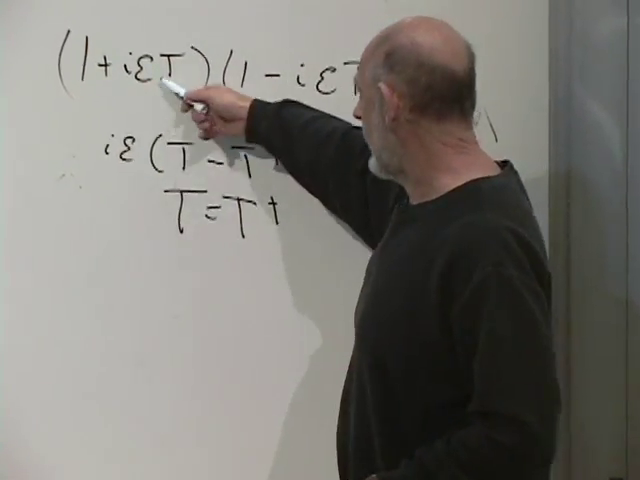
\includegraphics[width=0.62\textwidth]{lecture_04_figure_03.png}
\caption{Phép tính unita gần đơn vị kết thúc ở \(T=T^\dagger\).}
\lectureframe{00:23:28}
\end{figure}

Đối với các phép quay không gian, có ba toán tử sinh độc lập tuyến tính vì có ba trục độc lập cho các phép quay vô cùng bé. Một phép quay nhỏ quanh một hướng bất kỳ được ghép từ các phép quay nhỏ quanh \(x\), \(y\) và \(z\). Các toán tử sinh tương ứng là các toán tử mômen góc \(J_x,J_y,J_z\). Các giao hoán tử của chúng mã hóa tính không giao hoán của các phép quay,
\begin{equation}
[J_i,J_j]=i\epsilon_{ijk}J_k.
\label{eq:l4-angular-momentum-algebra}
\end{equation}
Từ đó, các phép quay vô cùng bé lặp lại dựng nên một phép quay hữu hạn.

Ta đã dùng tính unita nhưng vẫn chưa dùng điều kiện định thức bằng một. Với mọi ma trận nhỏ \(m\),
\begin{equation}
\det(\boldsymbol 1+\epsilon m)
=1+\epsilon\,\operatorname{tr}m+O(\epsilon^2).
\label{eq:l4-det-expansion}
\end{equation}

\begin{figure}[htbp]
\centering
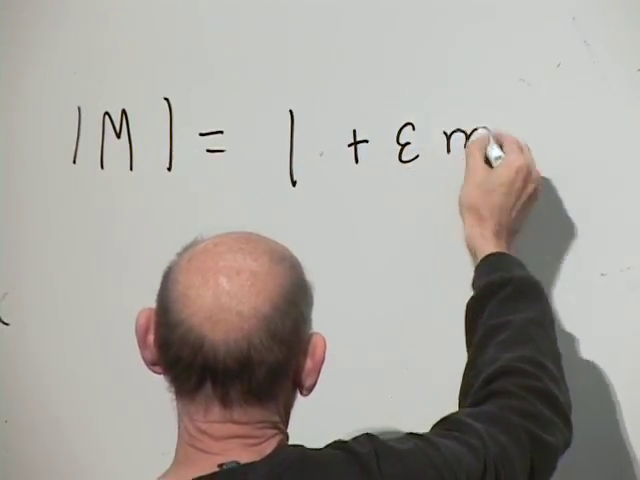
\includegraphics[width=0.62\textwidth]{lecture_04_figure_02.png}
\caption{Khai triển định thức bậc nhất ở bước đầu trên bảng.}
\lectureframe{00:21:51}
\end{figure}

Áp dụng Phương trình~\eqref{eq:l4-det-expansion} cho Phương trình~\eqref{eq:l4-infinitesimal-u},
\begin{equation}
\det U
=1+i\epsilon\,\operatorname{tr}T+O(\epsilon^2).
\end{equation}
Vì thế điều kiện unita đặc biệt đòi hỏi
\begin{equation}
\operatorname{tr}T=0.
\label{eq:l4-traceless-generator}
\end{equation}
Các toán tử sinh của \(SU(2)\) chính xác là các ma trận Hermite \(2\times2\) không vết. Không gian vectơ đó có số chiều là ba. Một cơ sở chuẩn được cho bởi các ma trận Pauli,
\begin{equation}
\begin{aligned}
\sigma_x&=
\begin{pmatrix}0&1\\1&0\end{pmatrix},
&
\sigma_y&=
\begin{pmatrix}0&-i\\i&0\end{pmatrix},
\\[0.4em]
\sigma_z&=
\begin{pmatrix}1&0\\0&-1\end{pmatrix}.
\end{aligned}
\end{equation}
Đối với biểu diễn spin một phần hai, có thể lấy \(J_i=\sigma_i/2\), nên một phép quay hữu hạn qua góc \(\theta\) quanh \(\hat{\boldsymbol n}\) là
\begin{equation}
U(\hat{\boldsymbol n},\theta)
=\exp\!\left(-i\theta\,
\hat{\boldsymbol n}\cdot\boldsymbol\sigma/2\right).
\end{equation}
\editorialnote{Số mũ hữu hạn là sự hoàn tất tiêu chuẩn của phần thảo luận về toán tử sinh vô cùng bé. Nguồn nhấn mạnh các phép quay nhỏ lặp lại hơn là viết công thức này tường minh.}

\begin{classroomqa}
\audiencequestion{Vậy có ba ma trận \(2\times2\) Hermite không vết độc lập phải không?
\lecturetimestamp{00:24:07}}
\lecturerresponse{Đúng. Chúng là ba ma trận Pauli. Với các ma trận unita đặc biệt \(3\times3\), số tương ứng là tám, và một cơ sở quy ước được cho bởi tám ma trận Gell-Mann.}
\end{classroomqa}

\begin{classroomqa}
\audiencequestion{Số tám đó có phải cũng chính là ``tám'' trong Bát đạo và tám gluon không?
\lecturetimestamp{00:24:43}}
\lecturerresponse{Toán học là cùng một loại lý thuyết biểu diễn \(SU(3)\), nhưng phải chỉ rõ đối xứng \(SU(3)\) nào đang tác dụng. Đối xứng hương vị kiểu Bát đạo trong lịch sử không phải là màu \(SU(3)\). Tám gluon thuộc biểu diễn adjoint của màu \(SU(3)\).}
\end{classroomqa}

\section{Từ SU(2) đến SU(3) màu}

Bây giờ tăng kích thước ma trận từ \(2\times2\) lên \(3\times3\). Một ma trận phức tổng quát
\(3\times3\) có chín phần tử phức, nên có mười tám tham số thực.
Điều kiện \(U^\dagger U=\boldsymbol 1\) cung cấp chín ràng buộc thực,
và \(\det U=1\) loại thêm một điều kiện nữa. Do đó
\begin{equation}
18-9-1=8.
\end{equation}
Có tám hướng vô cùng bé độc lập và tám toán tử sinh Hermite không vết. Khác với \(SU(2)\), nhóm này không phải là nhóm quay của không gian ba chiều thông thường. Nó là một đối xứng nội tác dụng lên màu.

Trước khi gán các biểu diễn đó cho quark, hãy nhắc lại cách các biểu diễn hợp thành phát sinh. Ghép hai hệ spin một phần hai lại với nhau và bỏ qua chuyển động quỹ đạo của chúng. Có bốn trạng thái tích, nhưng một phép quay không trộn lẫn cả bốn thành một biểu diễn bất khả quy duy nhất. Ba tổ hợp biến đổi như spin một,
\begin{align}
\ket{1,1}&=\ket{\uparrow\uparrow},\\
\ket{1,0}&=\frac{1}{\sqrt2}
(\ket{\uparrow\downarrow}+\ket{\downarrow\uparrow}),\\
\ket{1,-1}&=\ket{\downarrow\downarrow},
\end{align}
trong khi tổ hợp thứ tư biến đổi như spin không,
\begin{equation}
\ket{0,0}=\frac{1}{\sqrt2}
(\ket{\uparrow\downarrow}-\ket{\downarrow\uparrow}).
\end{equation}
Vì thế
\begin{equation}
\boldsymbol 2\otimes\boldsymbol 2
=\boldsymbol 3\oplus\boldsymbol 1.
\label{eq:l4-two-spin-decomposition}
\end{equation}
Các trạng thái thẳng hàng cho các thành viên \(m=\pm1\) của bộ ba, trạng thái đối xứng có hình chiếu bằng không hoàn tất nó, và tổ hợp phản đối xứng là singlet. Đây là logic tổng quát đằng sau việc cộng mômen góc và đằng sau việc kết hợp các biểu diễn màu.

Cùng sự phân biệt singlet--triplet ấy xuất hiện bất cứ khi nào hai bậc tự do spin một phần hai được ghép với nhau. Trong hiđrô nguyên tử, spin electron và proton tạo thành các trạng thái siêu tinh tế singlet và triplet. Ortho- và para-hiđrô dùng cùng lý thuyết biểu diễn đó cho spin hạt nhân của hai proton trong một phân tử \(H_2\).
\editorialnote{Nguồn dùng ``ortho- và para-hiđrô'' trong khi đang nói đến spin proton--electron trong một nguyên tử hiđrô. Phép phân rã toán học là đúng; ở đây các tên gọi cho trường hợp phân tử và nguyên tử được phân biệt để chính xác hơn.}

\subsection{Bộ ba và phản bộ ba}

Một quark đơn lẻ có ba biên độ màu. Trong một cơ sở đã chọn, viết
\begin{equation}
q=
\begin{pmatrix}
q_r\\q_g\\q_b
\end{pmatrix},
\qquad
q'=Uq,
\qquad U\in SU(3).
\label{eq:l4-quark-triplet}
\end{equation}
Ba phần tử có thể là các biên độ trạng thái của một quark hoặc ba toán tử trường tạo ra các quark đỏ, lục và lam. Nhóm trộn ba thành phần ấy. Một trạng thái ban đầu đỏ nói chung sẽ trở thành một chồng chập của đỏ, lục và lam sau một biến đổi màu. Biểu diễn cơ bản ba chiều này được gọi là \(\boldsymbol 3\).

Đối với một phản quark, nhóm tác dụng thông qua liên hợp phức của biểu diễn quark. Lấy liên hợp phức của Phương trình~\eqref{eq:l4-quark-triplet} ta được
\begin{equation}
\bar q'=U^*\bar q.
\end{equation}
Biểu diễn này được ký hiệu là \(\bar{\boldsymbol 3}\). Phép tương tự \(U(1)\) là rõ ngay: nếu trường electron nhận \(e^{i\theta}\), thì trường positron nhận \(e^{-i\theta}\). Các biến đổi màu của quark và phản quark là phiên bản không Abel của cặp liên hợp đó.

Gần đơn vị, nếu
\begin{equation}
U=\boldsymbol 1+i\epsilon T,
\end{equation}
thì
\begin{equation}
U^*=\boldsymbol 1-i\epsilon T^*.
\end{equation}
Vì vậy các toán tử sinh của phản bộ ba là \(-T^*\), tức các liên hợp với dấu ngược lại. Đây là nghĩa chính xác mà theo đó phản quark mang các điện tích màu đối nhau.

\begin{classroomqa}
\audiencequestion{Điều gì xảy ra với biểu diễn liên hợp phức trong trường hợp \(SU(2)\)?
\lecturetimestamp{00:36:19}}
\lecturerresponse{Doublet \(SU(2)\) là một trường hợp đặc biệt: liên hợp phức của nó tương đương với doublet ban đầu sau một phép đổi cơ sở cố định có dùng tensor epsilon phản đối xứng. Với \(SU(3)\), \(\boldsymbol 3\) và \(\bar{\boldsymbol 3}\) thực sự là các biểu diễn không tương đương.}
\end{classroomqa}
\editorialnote{Thuật ngữ chính xác về mặt toán học cho biểu diễn cơ bản \(SU(2)\) là giả thực, không phải thực. Phần trả lời này giữ nguyên sự phân biệt mà nguồn muốn diễn đạt đồng thời sửa lại thuật ngữ.}

\section{Kết hợp các biểu diễn màu}

Ký hiệu \(\otimes\) không có nghĩa là phép nhân thông thường của các con số viết bên cạnh nó. Nó có nghĩa là hai không gian trạng thái được kết hợp lại. Không gian tích tensor thu được sau đó được sắp xếp lại thành các phần không trộn lẫn với nhau dưới tác dụng của nhóm.

\subsection{Hai quark: \texorpdfstring{\(\boldsymbol 3\otimes\boldsymbol 3\)}{3 x 3}}

Hai quark có chín trạng thái cơ sở màu: đỏ--đỏ, đỏ--lục, đỏ--lam, và sáu cặp có thứ tự còn lại. Ta phân tách hai chỉ số màu thành một phần đối xứng và một phần phản đối xứng. Phần đối xứng có sáu thành phần độc lập; phần phản đối xứng có ba. Dưới \(SU(3)\),
\begin{equation}
\boldsymbol 3\otimes\boldsymbol 3
=\boldsymbol 6\oplus\bar{\boldsymbol 3}.
\label{eq:l4-three-times-three}
\end{equation}

\begin{figure}[htbp]
\centering
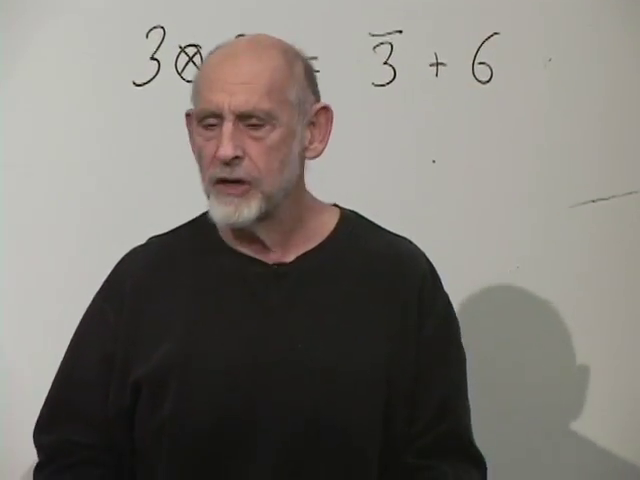
\includegraphics[width=0.68\textwidth]{lecture_04_figure_04.png}
\caption{Tích của hai quark tách thành một anti-triplet và một sextet.}
\lectureframe{00:39:33}
\end{figure}

Anti-triplet có thể được biểu diễn tường minh bằng cách co hai chỉ số quark với tensor epsilon bất biến,
\begin{equation}
(qq)^k_{\bar 3}
=\frac{1}{\sqrt2}\epsilon^{kij}q_iq_j.
\end{equation}
Đối tượng này có ba thành phần và biến đổi như một phản quark. Sáu tổ hợp đối xứng tạo thành sextet. Mệnh đề ở đây không phải là hai quark trở thành một phản quark theo nghĩa động lực học; mà là một sector của hàm sóng màu của chúng có cùng quy luật biến đổi như một phản quark.

\subsection{Một quark và một phản quark: \texorpdfstring{\(\boldsymbol 3\otimes\bar{\boldsymbol 3}\)}{3 x phản-3}}

Một trạng thái màu quark--phản quark có thể được xem như một ma trận \(3\times3\) \(M_i{}^j=q_i\bar q^j\). Mọi ma trận như vậy tách duy nhất thành phần vết và phần không vết của nó,
\begin{equation}
M=\frac{\operatorname{tr}M}{3}\boldsymbol 1
+\left(M-\frac{\operatorname{tr}M}{3}\boldsymbol 1\right).
\end{equation}
Vết là một thành phần bất biến đơn, còn phần không vết có tám thành phần. Do đó
\begin{equation}
\boldsymbol 3\otimes\bar{\boldsymbol 3}
=\boldsymbol 1\oplus\boldsymbol 8.
\label{eq:l4-three-times-threebar}
\end{equation}
Bỏ qua chuẩn hóa, singlet là
\begin{equation}
\ket{1}_{q\bar q}
=\frac{1}{\sqrt3}
(\ket{r\bar r}+\ket{g\bar g}+\ket{b\bar b}).
\end{equation}
Nó không thể biến đổi thành bất cứ tổ hợp nào khác vì nó là bất biến. Tám tổ hợp tuyến tính còn lại trộn lẫn với nhau. Chúng tạo thành biểu diễn adjoint, cũng là biểu diễn mà tám bộ sinh biến đổi theo.

\subsection{Ba quark}

Kết hợp thêm một quark thứ ba với phương trình~\eqref{eq:l4-three-times-three}. Nhánh phản bộ ba cho
\begin{equation}
\bar{\boldsymbol 3}\otimes\boldsymbol 3
=\boldsymbol 1\oplus\boldsymbol 8,
\end{equation}
nên tích ba quark chứa một singlet. Viết đầy đủ,
\begin{equation}
\boldsymbol 3\otimes\boldsymbol 3\otimes\boldsymbol 3
=\boldsymbol 1\oplus\boldsymbol 8\oplus\boldsymbol 8
\oplus\boldsymbol{10}.
\label{eq:l4-three-quark-full}
\end{equation}
Singlet màu là tổ hợp đỏ--xanh lục--xanh lam phản đối xứng hoàn toàn,
\begin{equation}
\ket{1}_{qqq}
=\frac{1}{\sqrt6}\epsilon^{ijk}\ket{q_iq_jq_k}.
\label{eq:l4-baryon-singlet}
\end{equation}
Vì \(\epsilon^{ijk}\) triệt tiêu bất cứ khi nào hai chỉ số trùng nhau, nên mọi số hạng khác không đều chứa một quark đỏ, một quark xanh lục và một quark xanh lam, với dấu luân phiên khi hoán đổi.

\begin{classroomqa}
\audiencequestion{Có phải các tổ hợp không singlet chỉ đơn thuần ít có khả năng xảy ra, nên có thể bỏ qua xác suất của chúng không?
\lecturetimestamp{00:46:02}}
\lecturerresponse{Không. Vấn đề là năng lượng, không phải xác suất nhỏ. Một trạng thái không singlet cô lập sẽ mang một trường màu ra tới khoảng cách lớn tùy ý và, trong chế độ giam hãm, sẽ đòi hỏi năng lượng không bị chặn trên. Động lực học đứng sau phát biểu đó sẽ được triển khai ở dưới.}
\end{classroomqa}

\subsection{Octet gluon}

Trường gluon biến đổi như octet trong Phương trình~\eqref{eq:l4-three-times-threebar}. Xét theo màu, nó mang một chỉ số triplet và một chỉ số anti-triplet, với phần vết singlet đã bị loại bỏ. Về mặt sơ đồ,
\begin{equation}
q\sim\boldsymbol 3,
\qquad
\bar q\sim\bar{\boldsymbol 3},
\qquad
G\sim\boldsymbol 8.
\end{equation}
Các ký hiệu này gọi tên các quy luật biến đổi; các hạt không theo nghĩa đen bằng các số nguyên 3 và 8.

Tổ hợp màu quark--phản quark thứ chín, tỉ lệ với ma trận đơn vị, là một singlet và không trộn với octet. Vì thế việc bỏ nó đi là nhất quán về mặt toán học: một trường gauge \(SU(3)\) là không vết và có tám thành phần thay vì chín thành phần của một trường gauge \(U(3)\).

\begin{classroomqa}
\audiencequestion{Vì sao tự nhiên bỏ đi gluon singlet phụ đó?
\lecturetimestamp{00:49:00}}
\lecturerresponse{Câu trả lời trực tiếp từ lý thuyết nhóm là singlet là một sector bất biến tách biệt, nên octet tự khép kín một cách nhất quán mà không cần đến nó. Lý do sâu hơn để chọn \(SU(3)\) thay vì \(U(3)\) không được suy ra ở đây; đó là một phần của cấu trúc gauge được suy ra từ hiện tượng học QCD.}
\end{classroomqa}

\section{Singlet màu dưới dạng hadron}

Các hạt tự do có khối lượng hữu hạn của tương tác mạnh là các singlet màu. Điều này không có nghĩa là quark hay gluon không có thực; nó có nghĩa là chúng không xuất hiện như các hạt tiệm cận cô lập. Các mô thức cơ bản để xây dựng singlet là
\begin{equation}
qqq,
\qquad
q\bar q,
\qquad
GG\ \text{and higher gluonic products}.
\end{equation}
Chúng lần lượt dẫn tới baryon, meson và glueball. Tích của vài đối tượng vốn đã không màu dĩ nhiên lại không màu, nên có thể xây dựng các trạng thái đa-hadron phức tạp hơn từ những thành phần này.

\begin{classroomqa}
\audiencequestion{Các singlet ba quark và quark--phản quark được gọi là gì, và gluon cũng có thể tạo thành singlet không?
\lecturetimestamp{00:51:38}}
\lecturerresponse{Một singlet ba quark là một baryon; một singlet quark--phản quark là một meson. Gluon cũng có thể kết hợp thành các singlet màu. Những trạng thái tương tác mạnh đơn giản nhất như vậy được gọi là glueball, và có thể có hơn hai gluon tham gia.}
\end{classroomqa}

Ba quark spin một phần hai luôn kết hợp thành một spin tổng thể bán nguyên, mặc dù mômen góc quỹ đạo có thể làm thay đổi giá trị bán nguyên nào xuất hiện. Meson quark--phản quark có spin nguyên. Glueball thuần gluon cũng có spin nguyên.

Đối với hai gluon, mệnh đề đầu tiên trên bảng chỉ là một phép đếm,
\begin{equation}
8\times8=1+63.
\end{equation}
Tổng cộng có 64 trạng thái màu; một tổ hợp là singlet và 63 tổ hợp còn lại thuộc các sector không singlet.

\begin{figure}[htbp]
\centering
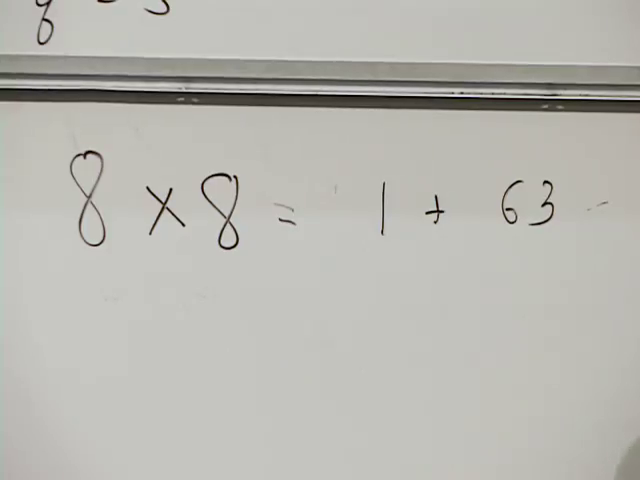
\includegraphics[width=0.68\textwidth]{lecture_04_figure_05.png}
\caption{Phép đếm trạng thái hai-gluon trên bảng: một singlet trong số 64 trạng thái.}
\lectureframe{00:53:44}
\end{figure}

Phân rã bất khả quy đầy đủ là
\begin{equation}
\boldsymbol 8\otimes\boldsymbol 8
=\boldsymbol 1\oplus\boldsymbol 8_S\oplus\boldsymbol 8_A
\oplus\boldsymbol{10}\oplus\overline{\boldsymbol{10}}
\oplus\boldsymbol{27}.
\label{eq:l4-eight-times-eight}
\end{equation}
Các số chiều cộng lại đúng:
\begin{equation}
1+8+8+10+10+27=64.
\end{equation}
Hai octet là những không gian con bất biến khác nhau, một đối xứng và một phản đối xứng dưới phép trao đổi hai thừa số adjoint. Singlet là kênh màu hai-gluon mà từ đó có thể tạo thành một trạng thái glueball.
\editorialnote{Trên bảng lúc đầu chỉ có \(8\times8=1+63\). Phần trao đổi sau đó trên lớp bổ sung các số chiều bất khả quy được liệt kê; các gạch trên và nhãn đối xứng được phục hồi ở đây theo ký hiệu \(SU(3)\) chuẩn.}

\subsection{Vì sao các điện tích quan sát được là số nguyên}

Điện tích của quark có hai loại,
\begin{equation}
Q_{\mathrm{up\text{-}like}}=+\frac23,
\qquad
Q_{\mathrm{down\text{-}like}}=-\frac13.
\end{equation}
Vì vậy ba quark có tổng điện tích nguyên: \(-1,0,+1,\text{ or }+2\),
tùy theo có bao nhiêu quark kiểu up. Tương tự, một quark và một phản quark có điện tích \(0\) hoặc \(\pm1\). Gluon không mang điện tích. Vì thế các singlet màu cơ bản được xây từ các biểu diễn quark quan sát được có điện tích nguyên, dù các thành phần của chúng mang điện tích phân số.

\begin{classroomqa}
\audiencequestion{Điện tích của quark lạ là bao nhiêu?
\lecturetimestamp{00:56:08}}
\lecturerresponse{Nó thuộc kiểu down, nên điện tích là \(-1/3\). Ba họ lặp lại cùng một mẫu điện tích: \((u,d)\), \((c,s)\) và \((t,b)\), với các điện tích \(+2/3\) và \(-1/3\) trong mỗi cặp.}
\end{classroomqa}

Tính singlet màu và điện tích nguyên liên hệ chặt chẽ với nhau đối với thành phần hạt này, nhưng chúng không phải là cùng một mệnh đề toán học. Tính nguyên ấy cũng dựa vào đúng các gán điện tích của Mô hình Chuẩn vừa được viết ra.

\begin{classroomqa}
\audiencequestion{Một singlet màu có phải là một trạng thái vướng víu không, và điều đó có cùng ý nghĩa như một cặp vướng víu trong một thí nghiệm Bell không?
\lecturetimestamp{00:56:58}}
\lecturerresponse{Hàm sóng màu singlet chắc chắn là vướng víu: nó là một chồng chập kết hợp, không phải tích của các màu riêng rẽ xác định. Về nguyên tắc các thành phần của nó có thể bị tách ra, nhưng sự giam hãm làm cho việc tách đó ngày càng tốn năng lượng và cuối cùng tạo ra các hadron mới. Vì thế đây không phải là một hệ thuận tiện cho thao tác kiểu Bell, dù trạng thái ấy là vướng víu.}
\end{classroomqa}

\section{Ý nghĩa của các phương trình tích tensor}

Đến đây, các bảng nhân xứng đáng được giải thích cụ thể hơn. Gọi \(\psi_i\) và \(\phi_j\) là các toán tử tạo ra hai đối tượng spin một phần hai; chúng có thể mô tả hai loại hạt, chẳng hạn một electron và một proton, hoặc hai bản sao của cùng một loại khi đã tính đến thống kê thích hợp. Mỗi chỉ số nhận hai giá trị. Bốn tích
\begin{equation}
\psi_\uparrow\phi_\uparrow,
\quad
\psi_\uparrow\phi_\downarrow,
\quad
\psi_\downarrow\phi_\uparrow,
\quad
\psi_\downarrow\phi_\downarrow
\end{equation}
sinh ra không gian tích tensor.

Nếu một phần tử nhóm tác dụng như \(U\) lên mỗi thừa số, thì nó tác dụng như \(U\otimes U\) lên tích. Theo thành phần,
\begin{equation}
\psi_i\phi_j
\longmapsto
U_i{}^kU_j{}^\ell\psi_k\phi_\ell.
\label{eq:l4-product-action}
\end{equation}
Đây là một biểu diễn bốn chiều, nhưng nó khả quy. Tổ hợp phản đối xứng
\begin{equation}
\frac{1}{\sqrt2}
(\psi_\uparrow\phi_\downarrow
-\psi_\downarrow\phi_\uparrow)
\end{equation}
được ánh xạ vào chính nó, còn ba tổ hợp đối xứng thì trộn lẫn với nhau. Trong cơ sở thích hợp với các tổ hợp đó, mọi ma trận của biểu diễn tích đều có dạng khối chéo,
\begin{equation}
D_{2\otimes2}(g)
\sim
\begin{pmatrix}
1&0\\
0&D_3(g)
\end{pmatrix}.
\label{eq:l4-spin-block-diagonal}
\end{equation}

\begin{classroomqa}
\audiencequestion{Một phương trình như \(\boldsymbol 3\otimes\boldsymbol 3=\bar{\boldsymbol 3}\oplus\boldsymbol 6\) biểu diễn thao tác nào?
\lecturetimestamp{00:57:51}}
\lecturerresponse{Vế trái tạo thành không gian trạng thái hợp thành. Nhóm tác dụng lên cả hai thừa số và vì thế trộn các trạng thái cơ sở của tích. Vế phải nói rằng một phép đổi cơ sở tách các trạng thái đó thành các tập bất biến: ba tổ hợp phản đối xứng biến đổi như một anti-triplet và sáu tổ hợp đối xứng biến đổi như một sextet. Dấu cộng có nghĩa là tổng trực tiếp của các phần, không phải phép cộng số học thông thường.}
\end{classroomqa}

\begin{classroomqa}
\audiencequestion{Làm sao ta biết 9 trạng thái tách thành \(3+6\), hay \(1+8\), thay vì, chẳng hạn, \(2+7\)?
\lecturetimestamp{01:04:39}}
\lecturerresponse{Chỉ đếm số chiều thì không thể quyết định cách tách. Ta phải biết \(SU(3)\) có những biểu diễn bất khả quy nào và xây dựng các không gian con bất biến, chẳng hạn bằng cách đối xứng hóa các chỉ số, phản đối xứng hóa chúng, hoặc tách phần vết khỏi phần không vết. Một sự phân loại đầy đủ đòi hỏi nhiều lý thuyết nhóm hơn; ở đây ta chỉ dùng các biểu diễn cần cho quark và gluon.}
\end{classroomqa}

Tensor epsilon bất biến làm cho việc xây dựng singlet trở nên minh bạch. Với \(SU(2)\),
\begin{equation}
\epsilon_{ij}U^i{}_kU^j{}_\ell
=(\det U)\epsilon_{k\ell}
=\epsilon_{k\ell}.
\end{equation}
Vì thế \(\epsilon_{ij}\psi^i\phi^j\) là bất biến. Với \(SU(3)\), phiên bản ba chỉ số cho
\begin{equation}
\epsilon_{ijk}U^i{}_aU^j{}_bU^k{}_c
=(\det U)\epsilon_{abc}
=\epsilon_{abc},
\end{equation}
điều này chứng minh tính bất biến của trạng thái ba-quark trong Phương trình~\eqref{eq:l4-baryon-singlet}.

\begin{classroomqa}
\audiencequestion{Có thể chỉ ra tường minh vì sao singlet không biến đổi không?
\lecturetimestamp{01:07:18}}
\lecturerresponse{Có. Hãy co tất cả các chỉ số cơ bản với tensor epsilon phản đối xứng hoàn toàn. Dưới phép biến đổi, tích các ma trận nhân epsilon với \(\det U\). Đối với một ma trận unita đặc biệt, định thức đó bằng 1, nên trạng thái đã co không đổi. Trong \(SU(2)\) điều này chứng minh singlet hai-spin; trong \(SU(3)\) nó chứng minh singlet ba-quark đỏ--lục--lam.}
\end{classroomqa}

\begin{classroomqa}
\audiencequestion{Phân rã đầy đủ của hai octet gluon là gì?
\lecturetimestamp{01:09:24}}
\lecturerresponse{Đó là phân rã trong Phương trình~\eqref{eq:l4-eight-times-eight}: một singlet, hai octet, một decuplet, một anti-decuplet và một biểu diễn 27 chiều. Có đúng một tổ hợp singlet màu của hai chỉ số octet.}
\end{classroomqa}

\begin{classroomqa}
\audiencequestion{Phân rã đầy đủ tương ứng đối với ba quark là gì?
\lecturetimestamp{01:11:51}}
\lecturerresponse{Câu trả lời cốt yếu về mặt vật lý là nó chứa một singlet. Hoàn tất phép cộng cho ta Phương trình~\eqref{eq:l4-three-quark-full}: một singlet, hai octet và một decuplet, tổng cộng \(1+8+8+10=27\) trạng thái.\editorialnote{Trong phần trao đổi này, giảng viên không nhớ phân rã đầy đủ của \(3\otimes3\otimes3\). Phần hoàn chỉnh chuẩn được cung cấp tường minh ở đây và được gắn nhãn tại đây thay vì quy cho câu trả lời bằng lời.}}
\end{classroomqa}

Ý tưởng tương tự mở rộng lên không gian hai gluon. Trong cơ sở tích tensor ngây thơ, \(SU(3)\) tác dụng thông qua các ma trận \(64\times64\). Trong một cơ sở thích nghi với các thành phần bất khả quy, các ma trận đó có dạng chéo khối,
\begin{equation}
\begin{aligned}
D_{8\otimes8}(g)
&\sim
\operatorname{diag}\bigl(
1,D_{8_S}(g),D_{8_A}(g),
\\
&\hspace{4.8em}
D_{10}(g),D_{\overline{10}}(g),D_{27}(g)
\bigr).
\end{aligned}
\end{equation}
Không có khối nào trộn với khối khác, mặc dù các trạng thái bên trong từng khối thì trộn lẫn với nhau.

\begin{classroomqa}
\audiencequestion{Phân rã tích tensor có phải chỉ là việc đổi sang một cơ sở trong đó ma trận biểu diễn lớn trở thành chéo khối không?
\lecturetimestamp{01:12:02}}
\lecturerresponse{Chính xác. Với hai spin, ma trận 4 chiều trở thành một khối singlet 1 chiều và một khối triplet 3 chiều. Với hai gluon, ma trận 64 chiều trở thành các khối có kích thước \(1,8,8,10,10,\text{ and }27\). Mỗi khối đều khép kín dưới mọi phép biến đổi nhóm.}
\end{classroomqa}

\begin{classroomqa}
\audiencequestion{Có tên gọi nào cho một trong những phần khép kín đó bên trong toàn bộ không gian tích tensor không?
\lecturetimestamp{01:14:55}}
\lecturerresponse{Đó là một không gian con bất biến mang một biểu diễn con. Khi không thể phân rã thêm nữa, nó mang một biểu diễn bất khả quy, hay irrep. Toàn bộ tích tensor là tổng trực tiếp của các thành phần bất khả quy đó.\editorialnote{Nguồn để ngỏ thuật ngữ được hỏi trong lớp. Trong câu trả lời, thuật ngữ chuẩn của lý thuyết biểu diễn được bổ sung.}}
\end{classroomqa}

\begin{classroomqa}
\audiencequestion{Khi các biểu diễn mười chiều không phải singlet và các biểu diễn khác bị gọi là không tồn tại, điều đó có nghĩa là phải hoàn toàn bỏ qua chúng hay không?\lecturetimestamp{01:15:36}}
\lecturerresponse{Chúng là những sector màu hợp lệ và có vai trò trong các phép tính trung gian, nhưng chúng không xuất hiện như những hạt cô lập có năng lượng hữu hạn trong phòng thí nghiệm. Chính sự giam hãm, chứ không phải sự thất bại của lý thuyết biểu diễn, ngăn chúng trở thành các trạng thái tiệm cận tự do.}
\end{classroomqa}

\section{Từ ý tưởng màu của Nambu đến sự giam hãm}

Ý tưởng về màu có trước công thức hóa cuối cùng của QCD. Ngay từ đầu những năm 1960, Yoichiro Nambu đã hiểu rằng một số lượng tử 3 giá trị ẩn có thể giải quyết một vấn đề nổi bật: quark mang điện tích phân số, nhưng không quan sát thấy hạt tự do nào mang điện tích phân số. Nếu các trạng thái vật lý bị buộc phải là singlet màu, thì quark xuất hiện trong các tổ hợp có điện tích nguyên như đã mô tả ở trên. Câu hỏi còn lại là câu hỏi động lực học: điều gì buộc mọi trạng thái tự do có năng lượng hữu hạn phải là singlet?

Bắt đầu với phép tương tự điện từ. Một điện tích và một điện tích trái dấu hút nhau. Đưa chúng lại gần nhau làm giảm năng lượng; còn ép các điện tích cùng dấu lại gần nhau thì cần thực hiện công. Bản thân trường chứa năng lượng dương,
\begin{equation}
E_{\mathrm{field}}
=\frac12\int d^3x\,\boldsymbol E^2
\end{equation}
trong các đơn vị tĩnh điện đơn giản. Một điện tích thuần để lại trường kéo dài rất xa ra ngoài hệ, trong khi một cặp trung hòa liên kết chặt chỉ có trường lưỡng cực tầm ngắn. Vì vậy, sự trung hòa loại bỏ năng lượng trường khỏi vùng bên ngoài.

Hãy tưởng tượng tăng độ ghép điện từ lên cực lớn. Mức phạt năng lượng trường đối với điện tích thuần sẽ trở nên lớn đến mức các đối tượng năng lượng thấp gần như đều trung hòa, và việc tách một thành phần mang điện ra có thể trở nên đòi hỏi năng lượng đến mức không khả thi. Nambu chuyển trực giác này sang màu: 8 điện tích màu là các nguồn của 8 trường gluon, nên năng lượng lớn của trường màu có thể cấm các trạng thái không singlet cô lập.

Trực giác ấy về cơ bản là đúng, nhưng QCD chứa một đặc trưng mới có tính quyết định. Photon không mang điện tích, còn gluon thì mang màu. Photon không phải là nguồn của trường điện từ cổ điển, và các phương trình Maxwell là tuyến tính: hai sóng điện từ chồng chất và đi xuyên qua nhau. Một gluon biến đổi trong octet màu, nên các gluon là nguồn của nhau và tương tác với nhau. Ngay cả các phần khác nhau của cùng một trường gluon cũng tương tác. Vì vậy trường gauge phi Abel là phi tuyến.

\subsection{Các ống thông lượng và thế tuyến tính}

Ở khoảng cách lớn, tự tương tác gluon ngăn không cho thông lượng màu loe ra như một trường lưỡng cực điện thông thường. Thông lượng bị ép vào một ống nối một quark với một phản quark. Cường độ trường và diện tích tiết diện của một ống dài xấp xỉ cố định, nên ống đó chứa một năng lượng trên mỗi đơn vị chiều dài xấp xỉ không đổi. Nếu \(\sigma\) ký hiệu lực căng dây này, thì
\begin{equation}
V(R)\simeq\sigma R+\text{constant}
\qquad (R\ \text{large}).
\label{eq:l4-linear-potential}
\end{equation}

\begin{figure}[htbp]
\centering
\includegraphics[width=0.78\textwidth]{lecture_04_figure_06.png}
\caption{Thông lượng màu bị bó lại thành một ống dài giữa một quark và một phản quark.}
\lectureframe{01:31:35}
\end{figure}

Điều này mạnh hơn thế Coulomb, vốn có độ lớn giảm theo \(1/R\). Kéo các nguồn màu ra xa hơn không làm lực suy yếu mãi; nó làm ống dài ra và tiếp tục cộng thêm năng lượng. Một điện tích màu đơn độc trong một thể tích vô hạn sẽ đòi hỏi một ống kéo dài vô tận và vì thế cần năng lượng không bị chặn trên. Đó chính là nội dung cụ thể của việc nói rằng chỉ các singlet màu mới có các trạng thái tiệm cận có năng lượng hữu hạn.
\editorialnote{Kí hiệu lực căng dây và thế ở khoảng cách lớn được viết tường minh làm cho phát biểu của nguồn, rằng một ống thông lượng đồng đều mang năng lượng đồng đều trên mỗi đơn vị chiều dài, trở nên định lượng.}

\subsection{Đứt dây và các jet}

Giả sử một va chạm cứng đánh trúng một quark bên trong một meson. Quark bắt đầu đi ra xa, nhưng ống thông lượng kéo giãn phía sau nó. Nó có thể mất động năng rồi bị kéo trở lại. Thường hơn, một khi năng lượng trường tích trữ đủ lớn, chân không tạo ra một cặp quark--phản quark mới. Phản quark mới làm đầu mút cho thông lượng gắn với quark đang thoát ra, còn quark mới làm đầu mút cho thông lượng gắn với phản quark ban đầu. Một singlet bị kéo giãn trở thành hai singlet ngắn hơn,
\begin{equation}
(q\bar q)_{\mathrm{stretched}}
\longrightarrow
(q\bar q)+(q\bar q).
\label{eq:l4-string-breaking}
\end{equation}

\begin{figure}[htbp]
\centering
\includegraphics[width=0.78\textwidth]{lecture_04_figure_07.png}
\caption{Sự tạo cặp làm đứt một ống thông lượng bị kéo giãn thành hai ống thông lượng singlet màu.}
\lectureframe{01:34:52}
\end{figure}

\begin{classroomqa}
\audiencequestion{Nếu một quark bị đánh trúng có đủ năng lượng để tiếp tục kéo giãn ống, thì ngoài việc bị kéo trở lại còn có thể xảy ra điều gì khác?
\lecturetimestamp{01:33:50}}
\lecturerresponse{Ống có thể bị đứt do sự tạo cặp quark--phản quark. Năng lượng của nó trở thành khối lượng và động năng của cặp mới. Các đầu mút nối lại thành hai singlet, nên quá trình này tạo ra thêm các meson chứ không tạo ra một quark cô lập.}
\end{classroomqa}

Nếu một trong các parton đó vẫn mang động lượng lớn, quá trình lặp lại. Kết quả là một thác các hadron singlet màu được chuẩn trực quanh hướng parton ban đầu: một jet. Sự chuyển hóa các quark và gluon giàu năng lượng thành các hadron được gọi là hadron hóa. Đối tượng mang màu khởi phát được suy ra từ jet, chứ không bao giờ được quan sát riêng rẽ.

\begin{classroomqa}
\audiencequestion{Sự đứt dây chỉ tạo ra meson, hay các hadron khác cũng có thể xuất hiện trong jet?
\lecturetimestamp{01:35:20}}
\lecturerresponse{Các hadron khác chắc chắn cũng có thể xuất hiện. Yêu cầu duy nhất về màu là các đối tượng quan sát được ở trạng thái cuối phải là singlet. Meson là hình dung đơn giản nhất cho một lần đứt, nhưng baryon, phản baryon và các tổ hợp singlet phức tạp hơn cũng có thể được tạo ra.}
\end{classroomqa}

Ba quark có thể cho thông lượng của chúng kết thúc tại một nút singlet màu. Bức tranh ba nhánh là đối ứng động lực học của tensor epsilon phản đối xứng trong Phương trình~\eqref{eq:l4-baryon-singlet}: không có thông lượng màu thuần nào thoát ra khỏi toàn bộ baryon.

\begin{figure}[htbp]
\centering
\includegraphics[width=0.72\textwidth]{lecture_04_figure_08.png}
\caption{Một nút thông lượng màu ba nhánh cho baryon, ở bên dưới hình phác họa đứt dây của meson.}
\lectureframe{01:36:12}
\end{figure}

\section{Các trường gauge, điện tích bảo toàn và Mô hình Chuẩn}

Ở mức độ hiện tại, có thể nhận ra một lý thuyết gauge là một lý thuyết trong đó một điện tích bảo toàn đóng vai trò nguồn cho một trường kiểu photon. Điện tích điện là nguồn của trường điện từ; 8 điện tích màu là nguồn của 8 trường gluon. Công thức sâu hơn làm cho đối xứng trở thành cục bộ và đưa vào một liên kết so sánh các trạng thái nội tại tại các điểm không-thời gian lân cận, nhưng cấu trúc đó không cần cho bức tranh giam hãm được phát triển ở đây.
\editorialnote{Công thức đối xứng cục bộ là nghĩa sâu hơn chuẩn của lý thuyết gauge mà nguồn có nhắc tới nhưng cố ý hoãn lại.}

Đối xứng, điện tích bảo toàn và thông lượng liên hệ chặt chẽ với nhau. Nếu các đường sức chỉ có thể kết thúc trên các điện tích, thì một nguồn không thể đơn giản biến mất trong khi thông lượng của nó vẫn còn gắn vào không đâu cả. Toàn bộ phần trường ở xa của nó cũng không thể biến mất tức thời, vì các biến đổi của trường lan truyền theo nhân quả. Ở dạng cục bộ, cùng một vật lý được biểu diễn bằng một phương trình liên tục,
\begin{equation}
\frac{\partial\rho}{\partial t}
+\boldsymbol\nabla\cdot\boldsymbol j=0,
\end{equation}
phương trình này nói rằng điện tích chỉ có thể rời khỏi một miền bằng cách chảy qua biên của miền đó. Lập luận bằng đường sức là bức tranh hình học của định luật bảo toàn cục bộ ấy.

Giờ ta có thể đặt kết quả này vào bên trong Mô hình Chuẩn. Màu đóng góp 8 phần tử sinh của \(SU(3)\) và 8 trường gluon tương ứng. Sector Abel cung cấp 1 phần tử sinh và 1 trường gauge. Ba phần tử sinh nữa thuộc về một \(SU(2)\) bổ sung, chứ không phải mômen động lượng không gian thông thường. Trước khi phá vỡ đối xứng, cấu trúc gauge là
\begin{equation}
SU(3)_c\times SU(2)_L\times U(1)_Y,
\end{equation}
với \(8+3+1=12\) phần tử sinh. Nhiệm vụ tiếp theo là hiểu \(SU(2)\) điện-yếu, rồi đến trường Higgs và cách photon quan sát được, \(W^\pm\) và \(Z\) xuất hiện.
\editorialnote{Nguồn gộp photon với 8 gluon và mô tả thừa số còn lại là \(SU(2)\times U(1)\). Trong Mô hình Chuẩn chưa phá vỡ đối xứng, thừa số Abel là siêu điện tích \(U(1)_Y\); photon chỉ xuất hiện sau khi trộn điện-yếu.}

Chuỗi lập luận trung tâm nay đã hoàn tất. Các nhóm trừu tượng tác dụng thông qua các biểu diễn; các phần tử sinh vi phân là các điện tích bảo toàn; quark, phản quark và gluon nằm trong \(\boldsymbol 3\),
\(\bar{\boldsymbol 3}\), và \(\boldsymbol 8\); các tích tensor xác định các hadron singlet; và trường gluon phi tuyến biến việc chọn singlet thành hiện tượng vật lý của sự giam hãm.